\glsresetall

\section{Addressing memory exhaustion \hspace{0.01cm} failures in Virtual Machines in a cloud environment}\label{section_memory_exhaustion}

With the expansion of the cloud computing usage over a wide range of areas and different kinds
of users, the cloud providers are taking full advantage of all their resources as much as they can.
Memory is the most expensive resource in terms of oversubscribing and this has resulted in high
price to the end user. Furthermore, performing swapping in \gls{vm} is expensive, so the cloud
provider usually do not offer any swapping space for its systems. As a consequence, when a \gls{vm}
runs out of memory, user processes are killed. This scenario in the cloud environment is
especially critical, since the user loses all of his/her execution time and, by extension,
the money invested in this computation. This paper addresses this critical problem by providing
a kernel extension that monitors the memory requirements of a \gls{vm} and prevents the out
of memory state by creating swapping space dynamically. The paper describes the design and
implementation of a preliminary prototype of this kernel extensions and evaluates its
performance.

\subsection{Introduction}
Cloud computing is increasingly being used for a wide range of applications and services
mainly due to its elasticity and new application opportunities \cite{Armbrust2009}. Because of this expansion,
cloud providers are facing a lot of pressure to make their physical resources handle high
user demands. This has resulted in oversubscribing resources by the cloud providers. The most
problematic resource to oversubscribe is memory, and indeed a cloud user is charged significantly
for memory. Memory unit cost is higher than any other cloud resource (\$0.028/GB versus \$0.012/CPU).
Cloud providers usually don’t provide any swap space in their instances due to high impact on
the performance of their systems. As a result, when a users \gls{vm} doesn’t have enough memory
to execute all the running applications, user processes are killed in order to keep the \gls{vm} alive.
This memory exhaustion failure results in a large financial loss for the user, since all the work done
by the killed processes is lost and all the money invested in these processes is wasted. Furthermore,
the user has to start a new, larger \gls{vm}, increasing the total cost for the user. In Linux systems,
processes are killed using the \gls{oom} Killer, a kernel module that prevents the Out Of Memory
machine state in the \gls{vm}. In this paper, we address this memory exhaustion problem by
introducing a kernel module called CUDSwap. This module is designed to avoid the \gls{oom} Killer
calls by adding more virtual memory to the system, i.e. adding more swapping space, when needed.
CUDSwap is a dynamic kernel module that monitors the amount of free system memory, and adds
swap space when the amount of free memory falls below a threshold. We have implemented a
prototype of this kernel module. Through some preliminary evaluation, we show that CUDSwap
prevents memory exhaustion failures. The paper describes the design, implementation and
preliminary evaluation of this prototype. In addition, we provide a cost benefit analysis of
using CUDSwap. By using a dynamic approach, CUDSwap uses the storage space only when it
is strictly needed. Furthermore, a lot of cloud users do not have enough computer knowledge
to create the swap space before running their program, so CUDSwap creates the swap space
for them. Another advantage of CUDSwap is in the case where a user unable to accurately
predict her program memory requirement. In some applications, it is hard to predict the
amount of memory they will need and the user may make an incorrect approximation that may
result in provisioning insufficient memory to its processes. CUDSwap enables such
processes to complete their execution. The remainder of this paper is organized as follows.
Section ~\ref{subme_related_work} provides a brief review of some important related work.
Section ~\ref{subme_oom} describes the details of how \gls{oom} Killer management
with respect to how it is invoked. Section ~\ref{subme_prev_oom_do} describes the
design approach of the system. Section ~\ref{subme_prev_oom_i} describes the
Linux implementation details of CUDSwap. Section ~\ref{subme_perf} discusses the
performance results. Section ~\ref{subme_cost} provides a cost benefit analysis.
Finally, Section ~\ref{subme_conclusio} discusses future directions and concludes the paper.

\subsection{Related Work}\label{subme_related_work}
Memory oversubscription has been extensively \hspace{0.01cm} studied from the cloud provider point of view, i.e.
the impact on the physical machine as a result of running several VMs on it. A wide range of
systems has been developed to face this challenge. In general, these systems fall into two
large categories depending on their approach: VM migration or Network Memory.
Systems using the VM migration approach are tailored to support sustained periods of
memory oversubscription. These systems provides support for reconfiguring a VM in a new
physical machine with enough resources to fulfill VM’s requirements. The main disadvantage of
this approach is the VM downtime. In order to be able to migrate the VM from one physical
machine to another, it has to be suspended in the old machine and resumed in the new one.
Although live migration techniques allow VM migration with minimal downtime, they still have
to face the network link saturation. Some examples of these systems are Xen \cite{Barham2003}, VMWare’s
VMotion \cite{Nelson2005} or SnowFlock \cite{Lagar-Cavilla2009}. On the other hand, systems using the Network Memory approach
are designed to support short memory overloads. These systems create a new memory hierarchy
by adding a new level of memory cache between the main memory and the disk, locating it across
the network. A large number of these systems use the concept of cooperative memory, which
consists of performing memory swapping across the network. The swapped out pages are stored
in remote page repositories. Earlier research has shown that cooperative memory has better
performance that disk swap \cite{Anderson1995}. However, the performance of these systems degrades significantly
when the duration of the overload increases due to network bottleneck. Examples of such
systems are Cellular Disco \cite{Govil2000}, Cooperative Caching \cite{Dahlin1994} or Nswap \cite{Newhall2003}. Recently, hybrid
systems have been proposed in order to take advantage of the VM migration and Network Memory
benefits. One such system is Overdriver \cite{Williams2011}, which monitors the memory overload and creates
adaptive thresholds. Based on these thresholds, the system decides between performing
Cooperative Swap or VM migration. Our CUDSwap work differs from these earlier approaches from
the memory overload point of view. While earlier approaches try to overcome the challenge of
memory exhaustion failure by managing the physical memory of the host machine, we analyze the
problem from the guest VM point of view. This way, we are giving the opportunity to the end
user to choose between different VM configurations knowing that her applications will be
completed and she can decide based on the performance-costs tradeoffs.

\subsection{Out-Of-Memory Linux Management}\label{subme_oom}
The \gls{oom} machine state is an undesired state where the Kernel is not able to allocate
more memory because there isn’t sufficient virtual memory available, i.e. the main memory
space and the swap space (in case of its existence) are full. In this scenario, the Linux
kernel tries to free up memory using the \gls{oom} Killer \footnote{\url{http://linux-mm.org/OOM_Killer}}. The \gls{oom} Killer is a
kernel system tailored to free up memory by killing processes. The \gls{oom} Killer is the
last resource used by the kernel to free up memory, since the kernel always tries to
maintain all the user processes alive. Killing processes is a critical operation, so the
\gls{oom} Killer has to decide which process is the most appropriate to be killed. The
\gls{oom} Killer is designed in a way that it tries to free up as much memory as possible
by killing as few processes as possible (only one if it is possible), and lose as little
work done (by killed processes) as possible. In order to do so, the \gls{oom} Killer
assigns a rank for each process following a set of rules. The rank for each process
is computed in a cumulative manner. Each process is continuously assigned points and
the process that has more points is more likely to be a candidate for termination. The
process rank is initialized with the amount of resident memory allocated by the process.
The independent allocated memory of each child process (excluding kernel threads) is then
added to the parent rank. After this, the process rank is decreased regularly by the CPU
and run times. This way, processes running for a long time are more likely to be kept alive,
fulfilling the premise of losing the minimum amount of work done. The rank of niced processes
is doubled because they are likely less important. Next, processes with the CAP\_SYS\_ADMIN or
CAP\_SYS\_RAWIO capabilities have their ranks reduced, since these processes have rights
to perform system administration operations and input/output operations, respectively.
They may leave the system in an inconsistent state if killed. Finally, the process rank is
shifted by the value in \texttt{/proc/<pid>/oom\_adj}, which is a user-defined value and
set to its parent value by default. The final result of following this procedure to determine
which process to kill when needed is that the processes that are killed are less important
(niced), use lots of memory, have not so far executed for long, and are not performing
any input/output operations.

\subsubsection{OOM Checklist}

Before calling the \gls{oom} Killer, the out of memory manager should go through a
checklist in order to ensure that the \gls{oom} Killer is called if and only if it is
necessary. This checklist performs the following steps:

\begin{enumerate}
    \item Is there enough swap space left? If yes, do not call \gls{oom}.
    \item Has it been more than five seconds since last failure? If yes, do not call \gls{oom}.
    \item Have we failed within the last second? If no, do not call \gls{oom}.
    \item Has it been ten failures at least in the last five seconds? If no, do not call \gls{oom}.
    \item Has a process been killed within the last five seconds? If yes, do not call \gls{oom}.
\end{enumerate}

This checklist ensures that the system is really out of memory and it is not, for example,
waiting for I/O to complete for pages swapped to disk.

\subsection{Preventing Out-Of-Memory State}\label{subme_prev_oom}

\subsubsection{Design Overview}\label{subme_prev_oom_do}

CUDSwap’s main goal is to avoid the calls to the \gls{oom} Killer by adding virtual
memory dynamically. In order to do that, CUDSwap is divided into three blocks. The
first block (mod\_hack\_brk module) is tailored to monitor the free memory of the
system and suspend the current process when there is a likelihood of memory exhaustion
failure. The second block (swap\_creator process) is responsible for creating a file,
format it as a swap space and activate it in order to allow the kernel to use it. Finally,
the third block (wake\_up module) is tailored to wake up the suspended processes.
Figure ~\ref{mefigure1} shows the overall behavior of the CUDSwap system. Each time
a process requests more memory to the kernel, the mod\_hack\_brk module intercepts the
requests and checks if the amount of free memory is below a system-dependent threshold.
If it is below the threshold, the module suspends the current process, stores the process
identifier in a file and notifies to the swap\_creator module that a new swap space is needed.
This module creates a new swap space and, when it finishes, reads the process identifiers
from the file created by the mod\_hack\_brk and sends them to the wake\_up module,
which wakes up those processes and allows them to continue their execution. This division
in three modules is convenient because it matches the three different steps carried out during
the VM checking and creation:

\begin{figure}[htbp]
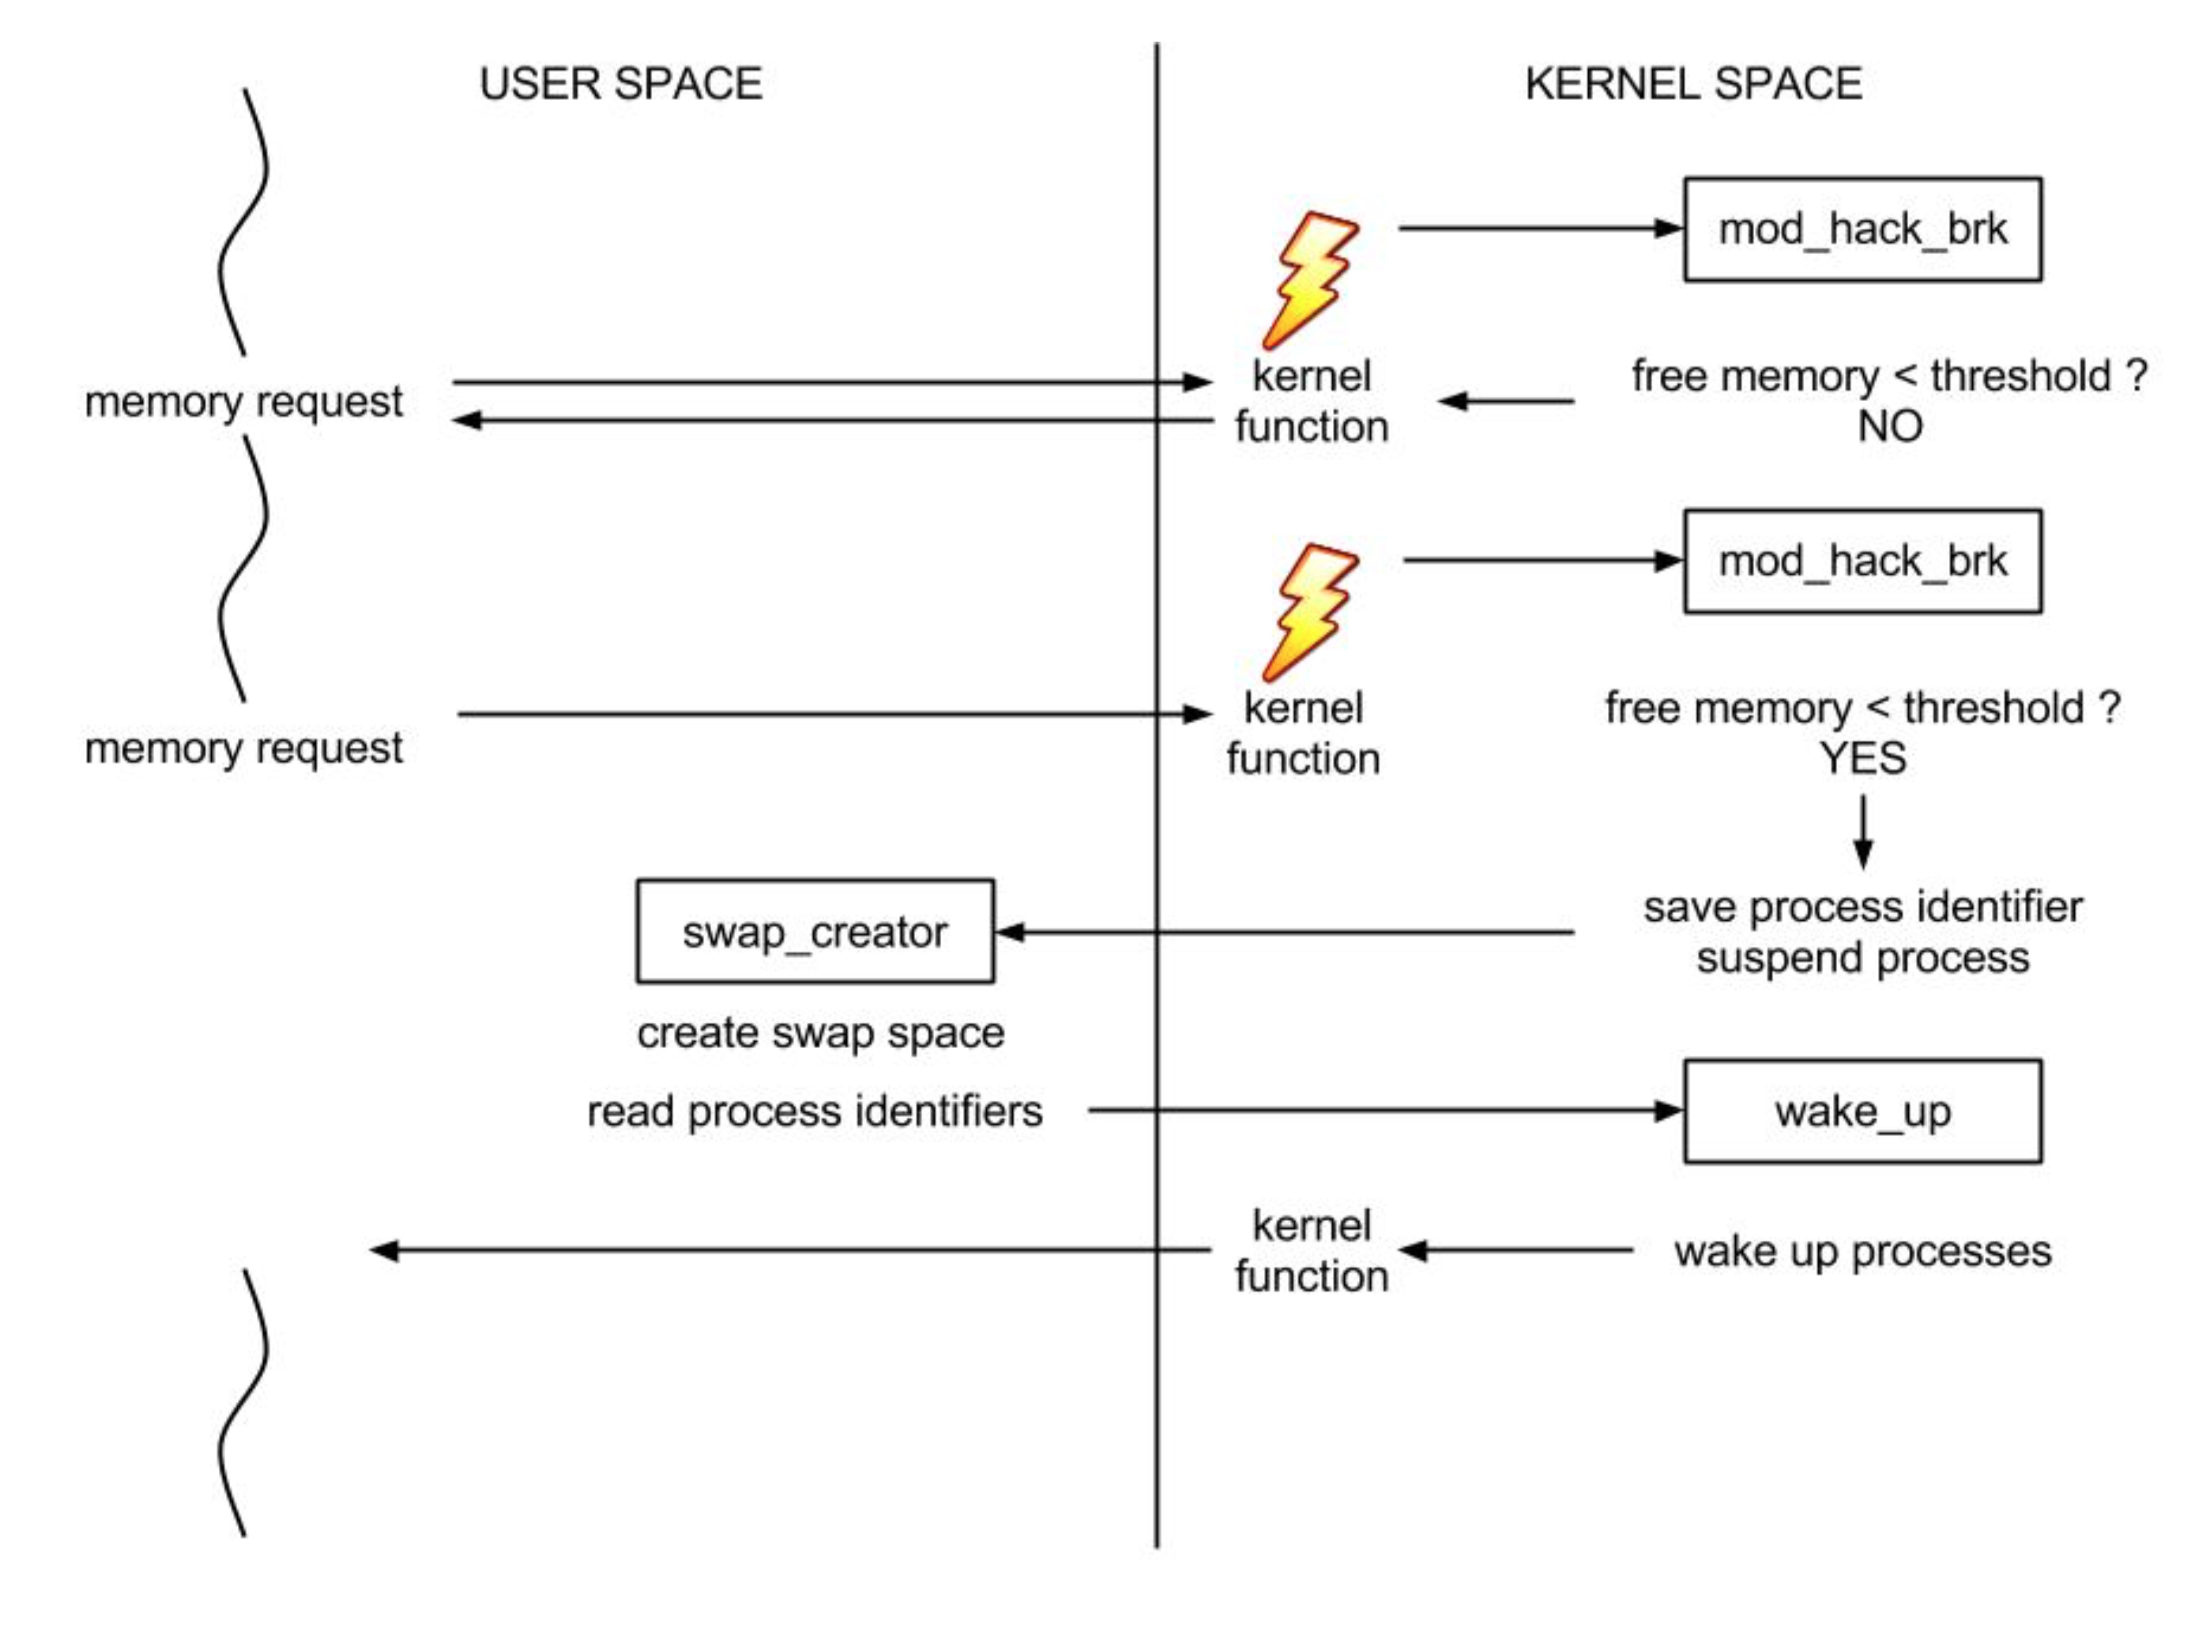
\includegraphics[width=\columnwidth]{chapter_memory_exhaustion_figures/Figure_1.png}
\caption[Design overview]{\textbf{Design overview.}}
\label{mefigure1}
\end{figure}

1) mod\_hack\_brk Module: The mod\_hack\_brk module is a kernel module that checks the
amount of free memory present in the system and checks if it is below a system-dependent
threshold. By default, the kernel sets a threshold in order to know if the machine is
in the out of memory state. This threshold is placed at 3\% of the total amount of virtual
memory present in the system. This way, the kernel has enough memory to run the \gls{oom}
Killer, if needed. The mod\_hack\_brk is more conservative and places the threshold at 7\%
of the total amount of system’s virtual memory. Hence, the swap\_creator process will have
enough memory to avoid the \gls{oom} Killer and create the swap space. In order to check the
amount of free memory we had to decide between two main directions: perform a periodic poll
or check each time a process requests more memory. The former has the main problem that it
will introduce an overhead in the system even if the system is idle. Another important drawback
of this solution is that we have to manage a trade-off between the time between polls and the
introduced overhead: if the polls are not sufficiently frequent, we may miss an out of memory
state and a user process will be killed. On the other hand, if the polls are too frequent,
the introduced overhead will be prohibitive. Thus, we decided to check the amount of free
memory each time a process requests more memory. When a process requests more memory to the kernel,
the the mod\_hack\_brk module intercepts this requests and, before any kernel function is executed,
checks the available memory in the system. This solution has the main drawback that it introduces
and overhead each time a process requests memory, but it avoids the trade-off described above regarding
the polling solution. In case the amount of free memory is below the threshold, the mod\_hack\_brk module
suspends the current process in order to prevent it from trying to allocate more memory. Then, the
module stores the process id in a configuration file and notifies to the swap\_creator process that
more swap space (i.e. virtual memory) is needed.

2) swap\_creator Process: The swap\_creator process is a process that runs with root
privileges in user space and its main function is to create a new swap space whenever
needed. During most of its lifetime, this process is sleeping and it is woken up only
when a new swap space is needed. The main reason why this is a process and this
functionality is not integrated within the mod\_hack\_brk module is that it is a bad
idea in general to open files from the kernel space. I/O operations are the source of
a large number of errors, and one of these errors in kernel space will cause the entire
system to crash. Hence, having all these operations in user space makes CUDSwap more robust.
Once this process is woken up, it performs four important steps. First, it creates a 2GB file
with no holes (i.e. it is not a sparse file and it is zeroed). Second, it creates a child
process that formats the created file as a swap space. Third, the swap creator process mounts
the created file as a swap space, increasing the amount of virtual memory. Finally, this process
reads the configuration file where the mod\_hack\_brk module had stored the sleeping process ids
and sends them to the wake\_up module.

3) wake\_up Module: The wake\_up module is a kernel module tailored to receive process
ids of sleeping processes and wake them up. The reason why this is a kernel module is
because the processes have been changed to sleeping mode in kernel space and, in order to
wake them up in a reliable manner, they should be woken up in kernel space.

\subsubsection{Implementation}\label{subme_prev_oom_i}

1) Intercepting memory requests: In the Linux kernel, there are two main system
calls that can be used by a process in order to modify its data segment: do\_mmap and
do\_brk. The most common system call used is do\_brk. In order to intercept the do\_brk calls,
we take advantage of Kprobes \cite{Krishnakumar2005}. Kprobes is a kernel debugger system that allows the
module programmer to add functions before and after a certain system call is executed.
This way, we can introduce a function before the do\_brk system call is executed and the
mod\_hack\_brk module can perform the needed checks to ensure the minimum free virtual
memory to avoid the OOM Killer calls.

2) Getting Memory Information: The easiest way to get the memory information is by
reading the \texttt{/proc/meminfo} file. Although reading a file from kernel space
is not recommended, the fact that this is a well-known file reduces the probabilities
of an I/O failure. However, there isn’t any easy way to manage files from the kernel
space because the standard libraries for manage files are not exported in kernel
space. Furthermore, in the newer kernel versions, the system calls to manage files
(\texttt{sys\_{open/read/write/close}}) are not exported. Hence, the only way to
manage file in kernel space is to go one step below and use low-level kernel functions,
using \texttt{linux/fs.h}. Since it is hard to manage files directly using this API,
we have created a simple library on top of this API that simplifies its usage and
it is as similar as possible to the standard C library API. This library is a bit
hackish because the functions defined in \texttt{linux/fs.h} expect that the buffer
address passed as parameter belongs to the user space. The addresses that we are
using are from kernel space, so these functions will fail. Our library fixes this
issue by marking our addresses as safe. This hack is done using the set\_fs function,
as shown below.

\begin{lstlisting}[language=C]
old_fs = get_fs();
set_fs(KERNEL_DS);
/* File operations */
set_fs(old_fs);
\end{lstlisting}

Once \hspace{0.01cm} we \hspace{0.01cm} get \hspace{0.01cm} our \hspace{0.01cm} library
for \hspace{0.01cm} file \hspace{0.01cm} management,\hspace{0.01cm} we can \hspace{0.01cm} parse the \texttt{/proc/meminfo}
file and get all the needed information. We have created a structure, mem info
struct, which stores all the relevant memory information and facilitates the out
of memory state detection. The contents of this structure are shown below.

\begin{lstlisting}[language=C]
typedef struct{
        unsigned long ram;
        unsigned long swap;
        unsigned long ram_free;
        unsigned long swap_free;
        unsigned long cached;
        unsigned long buffers;
        unsigned long total_vm;
        unsigned long free_vm;
        unsigned long sys_threshold;
        unsigned long committed_vm;
        unsigned int oc_ratio;
} mem_info_struct;
\end{lstlisting}

3) mod\_hack\_brk - swap\_creator Communication: The mod\_hack\_brk-swap\_creator
communication is challenging because we have to perform communication from the
kernel space to the user space (on the other direction, it is straightforward: system
calls). Furthermore, the swap creator process is a root process and the active
process during the execution of mod\_hack\_brk may be a non-root process without
privileges to send a signal to a root process. However, both problems are solved
because we have access to the signal primitives. Using the signal primitives, we
can provide the entire task struct of the receiving process, and our signals do not
pass the privileges checks.

4) swap\_creator - wake\_up Communication: The swap\_creator-wake\_up communication
is easier since the sender is in user space and the receiver in kernel space. In
this case, we have decided to use the procfs API in order to send each process
id to the wake up module. The wake up module creates a new entry in the \texttt{/proc}
filesystem, and the swap creator process simply opens it and writes the process
identifier of the sleeping process.

\subsection{Performance}\label{subme_perf}

CUDSwap is a set of modules that is always running in the system, so it will be
interesting to see how it affects the overall performance of the system. Since
CUDSwap mainly affects the performance of the do\_brk call, we have coded a simple
benchmark that stresses this situation.

Our benchmark consists of a program that allocates a large amount of memory 2GB in
our tests in chunks of 1KB. It then randomizes the character present in this memory
and counts the number of characters between 0 and 9. Finally, it frees the allocated
memory. These operations are performed 20 times. This simple benchmark executes a bunch
of do\_brk, so we can notice the overhead introduced by CUDSwap. It also accesses to
all the positions in the array multiple times, so we can also notice the performance
degradation due to swapping.

We performed our evaluation in Amazon EC2 \footnote{\url{ http://www.amazon.com/ec2}}. We have selected an M1 Medium instance
with the following characteristics: 2ECU, 3.75GB memory, 410GB storage, and Linux
kernel v3.0.14. Then, we ran our test, first without CUDSwap and next with CUDSwap
running on it. The total time to run our benchmark without CUDSwap was 1183.24 seconds,
and with CUDSwap, it was 1223.27 seconds. Thus the overhead introduced by CUDSwap is quite
low, only about 1.03X slower.

The second interesting performance comparison is running our benchmark in a smaller
instance with not enough memory, creating a new swapping space and allowing it to finish.
We chose an M1 Small instance with the following characteristics: 1ECU, 1.7GB memory,
160GB storage, and Linux kernel v3.0.14. The total run time in the small instance that
included adding swap space through CUDSwap was 8845.32 seconds. If a medium instance
is chosen instead, the run time is 1223.27 seconds. Thus, the benchmark in the smaller
instance is 7.23X slower due to low performance of swapping.

Finally, we also measured the time spent to create the swap space. This time was
418.43 seconds, which is much larger than we expected. This low performance is induced
by the fact that the storage in Amazon EC2 is in EBS volumes \footnote{\url{http://www.amazon.com/ebs}}, which are attached
to an instance through the network.

\subsection{Cost Analysis}\label{subme_cost}

Since CUDSwap is tailored for the cloud environment, its evaluation has to be based
on its derived costs too. First of all, we should derive the cost per resource unit
(ECU per hour, GB of memory per hour and GB of storage per hour). In order to do that,
we will solve systems of three equations of the type:

$$
C_{cpu} ∗ P_{cpu} + C_{mem} ∗ P_{mem} + C_{disk} ∗ P_{disk} = P_{instance}
$$

Here $C_i$ and $P_i$ are the configuration and price for the resource $i$ and $P_{instance}$
is the price of the instance.

Instead of picking only three instance types and solving only one system of equations,
we pick a subset of available instances in Amazon EC2 and solve all systems of three
equations resulting from all possible permutations. Table \ref{metable1} shows the selected
configurations and their price. We used a simple Python script to generate all systems,
their solutions and average them.

\begin{table}[htbp]
\centering
\caption[Selected instance configurations]{Selected instance configurations.}\label{metable1}
\begin{tabular*}{\textwidth}{ccccc}
\toprule
Name & $C_{cpu}$ & $C_{mem}$ & $C_{disk}$ & $C_{instance}$\\
\midrule
M1 Medium & 2 & 3.75 & 410 & 0.139\\
\midrule
M1 Large & 4 & 7.5 & 850 & 0.260\\
\midrule
M1 Extra-large & 8 & 15 & 1690 & 0.520\\
\midrule
M3 Extra-large & 13 & 15 & 0 & 0.580\\
\midrule
M3 Double extra-large & 26 & 30 & 0 & 1.160\\
\bottomrule
\end{tabular*}
\end{table}

Our calculations show that the cost for each ECU per hour is \$0.012, for each
GB of memory per hour is \$0.028 and for each GB of storage per hour is \$0. We
can see that the user is charged more for memory usage than for the CPU usage.
Hence, one possible way to save user’s money is to use a smaller instance with swap
space enabled.

If we pick as an example the test run from the previous section, where the benchmark
took 8845.32 seconds (2-3 hours) in the small instance and 1223.27 seconds ($<$1 hour)
in the medium instance, we can see that the user is charged \$0.195 (3 * 0.065) in the
small instance case and \$0.130 in the medium instance. Hence, if the user knows in
advance that his memory requirements will exceed that of small instance, it is cheaper to
run the code in the medium instance than in the smaller one with swap space.

However, the common case is one where the user doesn’t know in advance the total
memory requirements. In this case, the user typically runs his code in the smaller
instance and, when it gets killed, it terminates the small instance and runs his
code in the medium instance. Using the same example as above, we note that the user
would have spent a total amount of \$0.195 (1 hour for the small instance \$0.065 and 1 hour
for the medium one \$0.130). Then, we can see that the user would have spent the
same amount of money as running the code on a small instance with swap space. In
such a case, it is better for the user to use the small instance with swap space as
that avoids the hassle of moving the application from one instance to another.
Although in this case CUDSwap don’t save user’s money, it improves the user’s
experience because she doesn’t feel that she is wasting the money on the small
instance when it gets killed.

\subsection{Conclusion}\label{subme_conclusio}

In this paper we have described CUDSwap, a set of kernel modules that prevents the memory
exhaustion failure in virtual machines in cloud computing environment. We demonstrated
that the memory oversubscription is the most expensive resource in a cloud environment
and this cost is shifted to end user. Finally, we showed how CUDSwap could improve user’s
experience in a cloud environment.

The current prototype of CUDSwap is only a preliminary prototype and has a large scope
for improvement. The first source of improvement will be to obtain the memory
information directly from the kernel routines instead of reading the \texttt{/proc/info}
file. This will improve the out of memory state detection. With the current
implementation, we may miss an out of memory state if a process tries to allocate
more than 4\% of total memory with a single call. This is because we check for
memory threshold before a memory allocation takes place, but we do not take into
account how much memory the process is going to allocate.

The second source of improvement will be the way process identifiers are shared
between the mod\_hack\_brk and the swap\_creator process. Currently, this is done
through a configuration file, but one possible approach will be using the procfs
as in the wake\_up module case. This change will completely avoid the necessity
to open files in kernel space, making CUDSwap more robust and compliant with Linux
kernel development standards.

Finally, our current performance testing of CUDSwap is quite preliminary and
limited. We need to perform an extensive evaluation of CUDSwap with a wide variety
of applications having varied memory requirements. In particular, we need to test
UDSwap with standard memory benchmarks, and perform a cost benefit analysis. This
future tests can show cases where a smaller instance with swap space is cheaper
than a bigger instance with enough memory, as well as they will allow to characterize
the situations where CUDSwap is highly useful.
